\documentclass[a4paper,english,12pt]{article}   	% use "amsart" instead of "article" for AMSLaTeX format
\usepackage{geometry}                		% See geometry.pdf to learn the layout options. There are lots.
\geometry{letterpaper}                   		% ... or a4paper or a5paper or ...
%\geometry{landscape}                		% Activate for rotated page geometry
%\usepackage[parfill]{parskip}    		% Activate to begin paragraphs with an empty line rather than an indent
\usepackage{graphicx}				% Use pdf, png, jpg, or eps§ with pdflatex; use eps in DVI mode
								% TeX will automatically convert eps --> pdf in pdflatex		
\usepackage{amssymb}

%SetFonts

%SetFonts
\usepackage{%
	amsmath,%
	amsfonts,%
	amssymb,%
	amsthm,%
	hyperref,%
	url,%
	latexsym,%
	epsfig,%
	graphicx,%
	psfrag,%
	subfigure,%	
	color,%
	tikz,%
	pgf,%
	pgfplots,%
	pgfplotstable,%
	pgfpages,%
	proofs%
}

\usepgflibrary{shapes}
\usetikzlibrary{%
  arrows,%
	backgrounds,%
	chains,%
	decorations.pathmorphing,% /pgf/decoration/random steps | erste Graphik
	decorations.text,%
	matrix,%
  positioning,% wg. " of "
  fit,%
	patterns,%
  petri,%
	plotmarks,%
  scopes,%
	shadows,%
  shapes.misc,% wg. rounded rectangle
  shapes.arrows,%
	shapes.callouts,%
  shapes%
}

\theoremstyle{plain}
\newtheorem{thm}{Theorem}[section]
\newtheorem{lem}[thm]{Lemma}
\newtheorem{prop}[thm]{Proposition}
\newtheorem{cor}[thm]{Corollary}

\theoremstyle{definition}
\newtheorem{defn}[thm]{Definition}
\newtheorem{conj}[thm]{Conjecture}
\newtheorem{exmp}[thm]{Example}
\newtheorem{assum}[thm]{Assumptions}

%\theoremstyle{remark}
\newtheorem{rem}{Remark}
\newtheorem{note}{Note}

\makeatletter
\def\th@plain{%
  \thm@notefont{}% same as heading font
  \itshape % body font
}
\def\th@definition{%
  \thm@notefont{}% same as heading font
  \normalfont % body font
}
\makeatother
\date{}


\title{Lecture 13 : Topological Spaces and Continuous Functions}
\author{Parimal Parag}
\date{}							% Activate to display a given date or no date

\begin{document}
\maketitle
%\section{}
%\subsection{}
\section{}
\begin{defn}[Topology] A "topology" on a set $X$ is a collection $\mathcal{T}$ of subsets of $X$ having the following properties
\begin{enumerate}
\item $\phi$ and $X$ are in $\mathcal{T}$.
\item The union of the elements of any subcollection of $\mathcal{T}$ is in $\mathcal{T}$.
\item The intersection of any finite subcollection of $\mathcal{T}$ is in $\mathcal{T}$. A set $X$ for which a topology $\mathcal{T}$ has been specified is called a "topological space" $(X,\mathcal{T})$
\end{enumerate}
\end{defn}
\begin{defn}[Open Set] If $X$ is a topological space with topology $\mathcal{T}$, we say that a subsets $U$ of $X$ is an "open set" of $X$ if $U$ belongs to the collection of $\mathcal{T}$.
\end{defn}
\begin{exmp} 
 Let $X$ be any set, then its power set $\mathcal{P}(X)$ is a topolgy and is called as ``discrete topology''.  While topology $\mathcal{T} =\{\phi,X\}$ is called ``indiscrete topology'' or ``trivial topology''.
\end{exmp}
\begin{exmp} 
 Let $X$ be a set, and let $\mathcal{T}_f = \{U\subseteq X|X-U\text{ is finite or }X-U=X\}$. Prove that $\mathcal{T}_f$ is a topology on $X$.
 \begin{proof}
  Both $\phi$ and $X$ are in $\mathcal{T}_f$ since $X-\phi =X$ and $X-X$ is finite. Let $\{U_i\}$ be a indexed family of nonzero elements of $\mathcal{T}_f$. Now to show that the union of any subcollection $\mathcal{I}$ of $U_i$ is in $\mathcal{T}_f$ $$X-\bigcup_{i\in\mathcal{I}}U_i=\bigcap_{i\in\mathcal{I}}(X-U_i)\subseteq (X-U_i).$$ Since $X-U_i$ is finite hence union of any subcollection of $U_i$ is in $X$. Let $U_1,\ldots,U_n$ denote the finite nonzero elements of $X$. To show that their intersection is in $X$ $$X-\bigcap_{i\in\mathcal{I}}U_i=\bigcup_{i\in\mathcal{I}}(X-U_i),$$
  since it is a finite union of finite sets hence it is also finite. 
 \end{proof}
 \end{exmp}
 
\begin{exmp} Let $X=\{a,b,c\}$. The different topologies correspoding to $X$ are shown in the following figure:
\begin{figure}[!h]
 \centering
 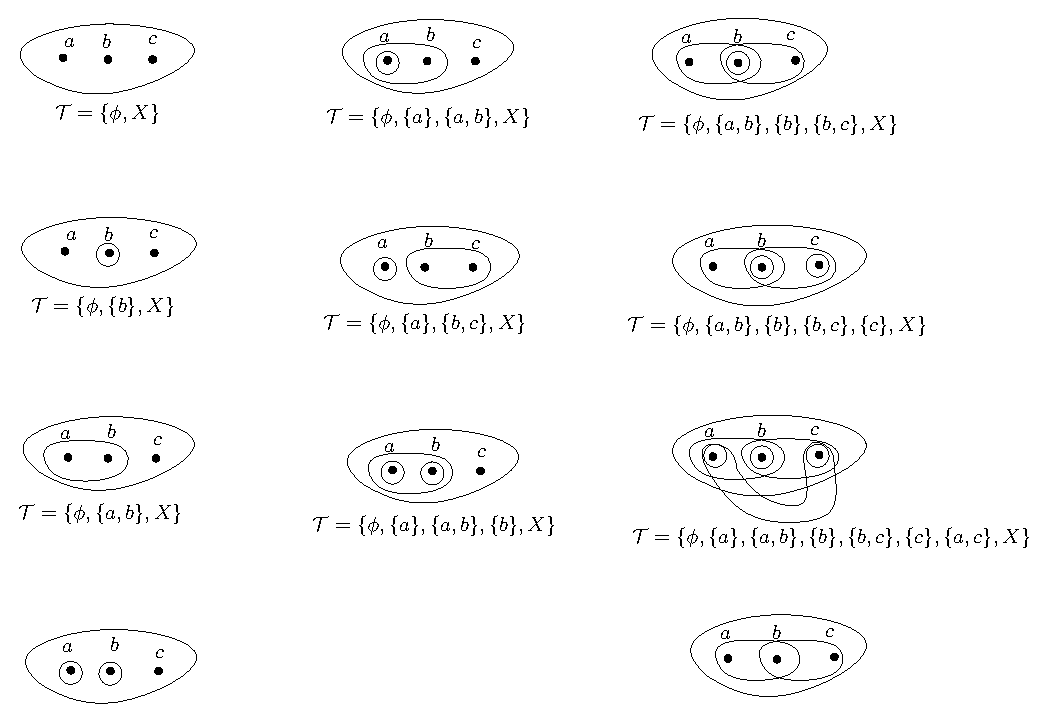
\includegraphics[height=3.5in]{fig133.eps}
\end{figure}

In the above, last two are not topologies.
\end{exmp}

\begin{exmp} 
 Let $X$ be a set and $\mathcal{T}_c=\{U\subseteq X: X-U \text{ countable or } X-U =X  \}$. Prove that $\mathcal{T}_c$ is a topology.
\end{exmp}
\begin{proof}
 
\end{proof}

\begin{defn}
 Let $\mathcal{T}$, $\mathcal{T}'$ be topologies on set $X$. If $\mathcal{T}\subseteq\mathcal{T}'$, we say that $\mathcal{T}'$ is ``finer'' than $\mathcal{T}$, and if  $\mathcal{T}\varsubsetneq\mathcal{T}'$, then ``strictly finer'', we say $\mathcal{T}$ is ``coarser" or ``strictly coarser" in these two cases, respectively. We say that $\mathcal{T}$ is comparable to $\mathcal{T}'$ if either
 $\mathcal{T}\varsubsetneq\mathcal{T}'$ or $\mathcal{T}' \varsubsetneq\mathcal{T}$.
\end{defn}
\begin{defn}
 If $\mathcal{T}\varsubsetneq\mathcal{T}'$, then we say that $\mathcal{T}'$ is ``larger" than $\mathcal{T}$, and $\mathcal{T}$ is ``smaller'' than $\mathcal{T}$
\end{defn}

\section{Basis for a Topology}
\begin{defn}
 If $X$ is a set, a ``basis" for a topology on $X$ is a collection $\mathcal{B}$ of subsets of $X$ (called ``basis" elements) such that 
 \begin{enumerate}
  \item $\forall x\in X, \exists B\in \mathcal{B}$ s.t. $x\in \mathcal{B}$.
  \item If $x\in B_1\bigcap B_2$, where $B_1, B_2 \in \mathcal{B}$ then $\exists B_3 \in \mathcal{B}$ s.t. $x\in B_3\subseteq B_1\bigcap B_2$.
 \end{enumerate}
\end{defn}
 If $\mathcal{B}$ satisfies these two conditions, we define the topology $\mathcal{T}$ generated by $\mathcal{B}$ as follows. A subset $U$ of $X$ is called open in $X$ if for each $x\in U, \exists B\in \mathcal{B}$ s.t. $x\in B\varsubsetneq U$. 
 Note: $\mathcal{B}\subseteq\mathcal{T}$.
 
 Next, we prove that the collection $\mathcal{T}$ generated by basis $\mathcal{B}$ is indeed a topology on $X$. First, we check that both $\phi$ and $X$ belongs to $\mathcal{T}$. Let $U$ be an emplty set, in this case $U$ vaccuously belongs to $\mathcal{T}$. Similarly $\forall x\in X, \exists B$ s.t. $x\in B\varsubsetneq X$. Next, to prove that the union of the elements of any subcollection of $\mathcal{T}$ is in $\mathcal{T}$, we take an indexed family $\bigcup_{i\in \mathcal{I}}U_i$ of elements of $\mathcal{T}$  and show that $\bigcup_{j\in \mathcal{J}}U_j$ is in $\mathcal{T}$. For each $x\in U$, there exists index $j\in J$ such that $x\in U_j$. Since $U_j \varsubsetneq \mathcal{T}$ there exists basis element $B$ such that $x\in B$ and $B\varsubsetneq U_j$. Thus $x\in B$ and $B\varsubsetneq U$, so $U\varsubsetneq\mathcal{T}$ by definition. 
 
 Let $U_1$ and $U_2$  be finite subcollections of $\mathcal{T}$. Now, first we want to show that $U_1\bigcap U_2 $ belongs to $\mathcal{T}$. Let $x\in U_1\bigcap U_2 $, we can choose a basis elements $B_1$ and $B_2$ such that $x\in B_1$ and $x\in B_2$, also $ B_1\varsubsetneq U_1$ and $B_2\varsubsetneq U_2$. Using the second condition in the definition of the basis we can choose a basis element $B_3$ such that $x\in B_3$ and $B_3\varsubsetneq B_1\bigcap B_2$. Then $x\in B_3$ and $B_3\varsubsetneq U_1\bigcap U_2$, thus $U_1\bigcap U_2$ belongs to $\mathcal{T}$, by definition. Using induction we can show that any arbitrary intersection belongs to $\mathcal{T}$.

\begin{figure}[!h]
 \centering
 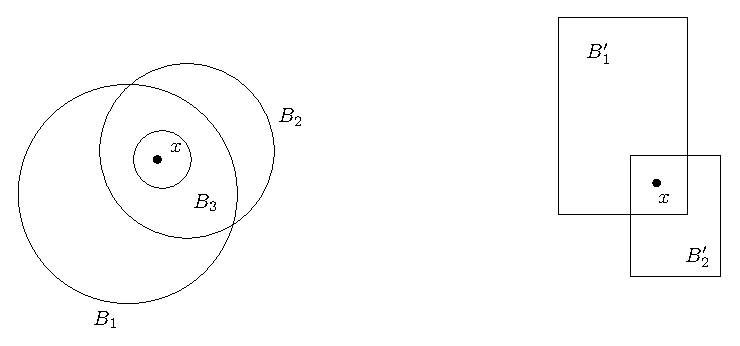
\includegraphics[height=2in]{fig134.eps}
\end{figure}

\begin{exmp}
 As shown in above figure, consider the collection of all circular regions (interiors of circles) $\mathcal{B}$. $\mathcal{B}$ is a basis. 
\end{exmp}
\begin{exmp}
 $\mathcal{B}'$ collection of rectangular elements is also a basis. 
\end{exmp}
\begin{exmp}
 Let X be any set, then collection of all one-point subsets is basis for ``discrete topology" on $X$.
\end{exmp}
 \begin{lem}
Let $X$ be a set, and $\mathcal{B}$ be a basis for topology $\mathcal{T}$ on $X$. Then $\mathcal{T}$ equals the collection of all unions of elemetns of $\mathcal{B}$.
\end{lem}
\begin{proof} Since $\mathcal{B}\varsubsetneq\mathcal{T}$ and $\mathcal{T}$ is a topology then collection of all union of $\mathcal{B}$ is in $\mathcal{T}$. Now, we have to show $\mathcal{T}\subseteq \text{ collection of all union of elements of } \mathcal{B}$. Let $U\in \mathcal{T}$, let $x\in U$, choose $B_x\in \mathcal{B}$ s.t. $x\in B_x\subseteq U$. Then $U=\bigcup_{x\in U}B_x$.
\end{proof}


\end{document}  